\chapter{Resultados} \label{cap:resultados}

Este capítulo apresenta os resultados de cada etapa do \textit{pipeline} descrito no Capítulo~\ref{metodologia}, na ordem em que foram executadas. Todos os números foram extraídos dos arquivos de resultados da execução com semente 42 e podem ser reproduzidos com o código disponibilizado.

% =============================================================================
\section{Análise Exploratória dos Dados}
\label{sec:res_aed}
% =============================================================================

Apenas \textit{AG\_Ratio} teve valores ausentes (4 registros, 0,69\% da base), e foram encontrados 13 registros exatamente duplicados. A base tem 416 doentes (71,4\%) e 167 saudáveis (Figura~\ref{fig:eda_distribuicao_alvo}), e 441 homens (75,6\%) e 142 mulheres. A proporção de doentes é maior entre os homens (73,5\%) do que entre as mulheres (64,8\%), o que impede comparar diretamente entre os sexos métricas que dependem da prevalência, como a precisão.

As maiores diferenças entre as classes (Tabela~\ref{tab:medias_classe}) estão nas bilirrubinas (média da direta cerca de 4,9 vezes maior nos doentes, e da total, 3,6 vezes) e nas aminotransferases (cerca de três vezes); \textit{Total\_Proteins} quase não difere (6,46 contra 6,54). Nos \textit{boxplots} (Figura~\ref{fig:eda_boxplots}), porém, as caixas de doentes e saudáveis se sobrepõem em todas as variáveis, de modo que nenhum exame sozinho separa bem as classes, o que motiva o uso de modelos multivariados.

Houve correlação forte em três pares (Figura~\ref{fig:eda_correlacao}): bilirrubina total e direta ($r = 0{,}874$), ALT e AST ($r = 0{,}792$) e proteínas totais e albumina ($r = 0{,}783$), todas com explicação fisiológica (Seção~\ref{sec:fund_figado}). Além disso, \textit{Total\_Proteins}, \textit{Albumin} e \textit{AG\_Ratio} são redundantes: como a globulina é a diferença entre proteínas totais e albumina, quaisquer duas delas determinam a terceira. Essa redundância reaparece na interpretação dos modelos (Seções~\ref{sec:res_coef_lr} e~\ref{sec:res_shap_global}).

% =============================================================================
\section{Pré-processamento}
\label{sec:res_preproc}
% =============================================================================

A remoção das duplicatas deixou 570 pacientes (406 doentes e 164 saudáveis). A transformação logarítmica reduziu a assimetria das cinco variáveis de 3,17--10,50 para 1,24--1,72 (Tabela~\ref{tab:assimetria_log}). A divisão resultou em 457 pacientes no treino e 113 no teste (71,1\% e 71,7\% de doentes; 32 mulheres e 81 homens no teste). Os quatro valores ausentes caíram no treino e foram imputados com a mediana (1,00).

\subsection{Reamostragem com SMOTE}
\label{sec:res_smote}

No treino completo, o SMOTE gerou 132 amostras sintéticas de pacientes saudáveis, e a razão entre as classes passou de cerca de 2,5:1 (325 doentes e 132 saudáveis) para 1,2:1 (325 e 264) (Figura~\ref{fig:res_smote}). As médias das amostras sintéticas ficaram a menos de 0,05 desvio-padrão das dos saudáveis originais, e apenas uma delas precisou ter o valor de \textit{Gender} corrigido.

\begin{figure}[htbp]
\centering
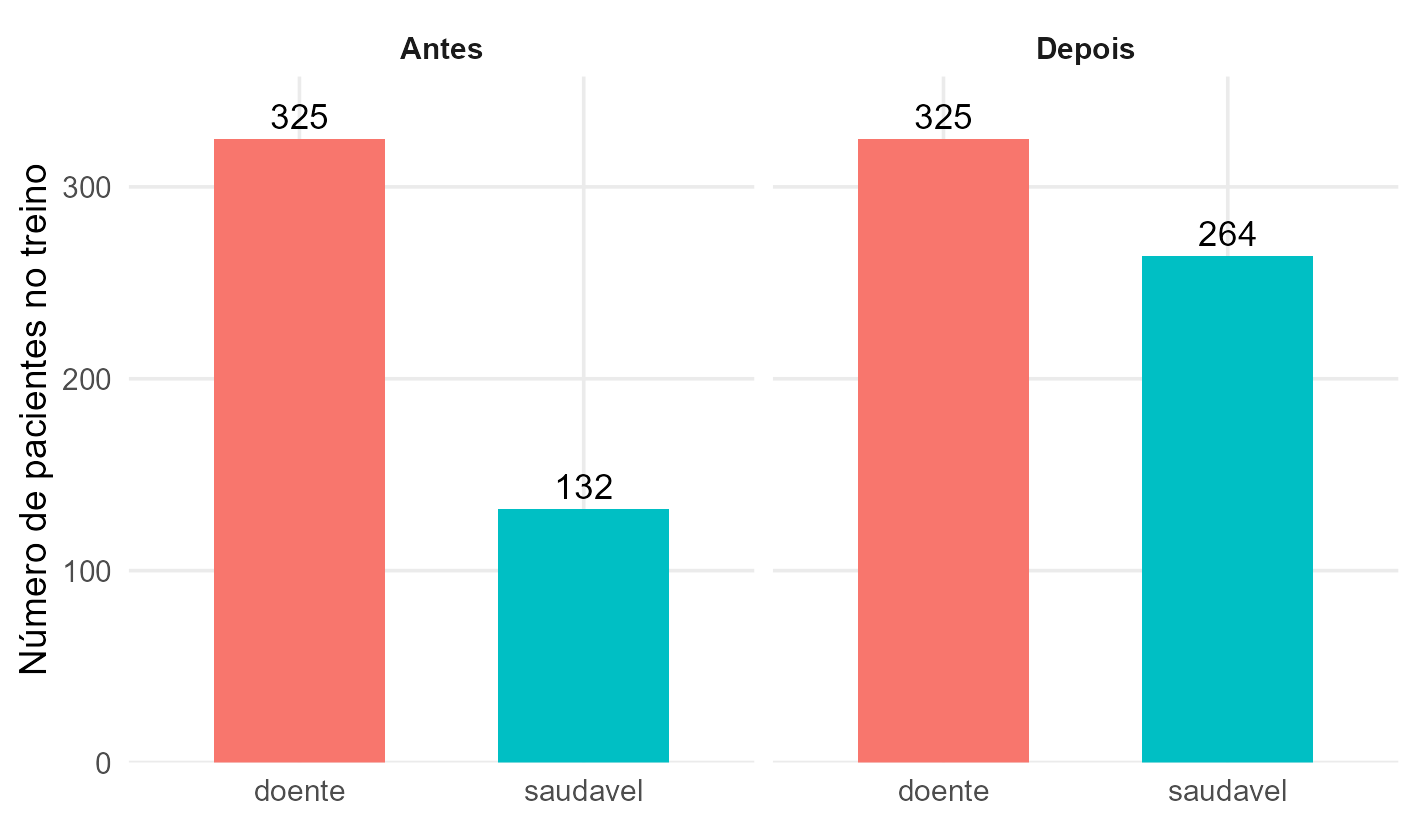
\includegraphics[width=0.6\textwidth]{figuras/cap5-resultados/smote_antes_depois.png}
\caption{Distribuição das classes no conjunto de treino antes e depois do SMOTE.}
\label{fig:res_smote}
\end{figure}

% =============================================================================
\section{Treinamento e Validação Cruzada}
\label{sec:res_cv}
% =============================================================================

\subsection{Hiperparâmetros Selecionados}

Os hiperparâmetros selecionados (Tabela~\ref{tab:res_hiper}) correspondem a modelos simples. No \textit{Random Forest}, venceu \texttt{mtry} = 1, isto é, cada divisão considera uma única variável sorteada. O XGBoost usa só 24 árvores, \texttt{gamma} alto (7,33), que só aceita divisões que reduzam bastante a perda, e cerca de um terço das variáveis por árvore. O LightGBM usa 200 árvores com no máximo quatro folhas e taxa de aprendizado baixa. Em uma base pequena e com classes sobrepostas, a validação cruzada favoreceu modelos que capturam poucos padrões, o que tem consequências para a interpretabilidade (Seção~\ref{sec:res_shap_global}).

\begin{table}[htbp]
\centering
\caption{Hiperparâmetros selecionados pela busca aleatória (maior AUC-ROC média na validação cruzada).}
\label{tab:res_hiper}
\begin{tabular}{lll}
\hline
\textbf{Modelo} & \textbf{Hiperparâmetro} & \textbf{Valor selecionado} \\
\hline
\textit{Random Forest} & \texttt{mtry} & 1 \\
 & \texttt{ntree} & 500 (fixo) \\
\hline
XGBoost & \texttt{nrounds} & 24 \\
 & \texttt{max\_depth} & 4 \\
 & \texttt{eta} & 0,226 \\
 & \texttt{gamma} & 7,33 \\
 & \texttt{colsample\_bytree} & 0,345 \\
 & \texttt{min\_child\_weight} & 16 \\
 & \texttt{subsample} & 0,485 \\
\hline
LightGBM & \texttt{num\_leaves} & 4 \\
 & \texttt{learning\_rate} & 0,0116 \\
 & \texttt{nrounds} & 200 \\
 & \texttt{feature\_fraction} & 0,57 \\
 & \texttt{min\_data\_in\_leaf} & 40 \\
\hline
\end{tabular}
\end{table}

\subsection{Desempenho na Validação Cruzada}

A Regressão Logística obteve a maior AUC-ROC média (0,753), e os três \textit{ensembles} ficaram praticamente empatados entre 0,720 e 0,725 (Tabela~\ref{tab:res_cv} e Figura~\ref{fig:res_cv}). A variação entre partições, porém, foi muito maior que essas diferenças: no \textit{Random Forest}, a AUC foi de 0,581 a 0,810.

\begin{table}[htbp]
\centering
\caption{AUC-ROC nas 15 partições de validação e sensibilidade e especificidade médias no limiar de 0,5.}
\label{tab:res_cv}
\begin{tabular}{lcccccc}
\hline
\textbf{Modelo} & \textbf{AUC média} & \textbf{DP} & \textbf{Mín.} & \textbf{Máx.} & \textbf{Sens.} & \textbf{Espec.} \\
\hline
Regressão Logística    & 0,753 & 0,054 & 0,654 & 0,836 & 0,667 & 0,694 \\
\textit{Random Forest} & 0,723 & 0,074 & 0,581 & 0,810 & 0,751 & 0,515 \\
XGBoost                & 0,725 & 0,064 & 0,616 & 0,827 & 0,701 & 0,639 \\
LightGBM               & 0,720 & 0,064 & 0,607 & 0,792 & 0,685 & 0,659 \\
\hline
\multicolumn{7}{l}{\footnotesize DP: desvio-padrão entre as 15 partições.} \\
\end{tabular}
\end{table}

\begin{figure}[htbp]
\centering
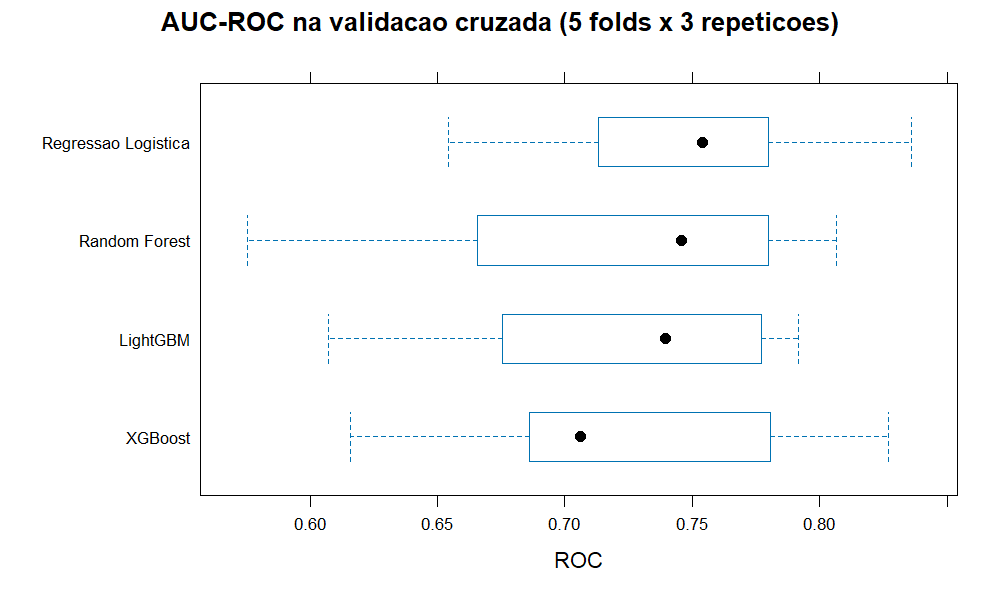
\includegraphics[width=0.75\textwidth]{figuras/cap5-resultados/cv_comparacao_modelos.png}
\caption{Distribuição da AUC-ROC nas 15 partições de validação. Cada ponto é uma partição, e o losango indica a média.}
\label{fig:res_cv}
\end{figure}

\subsection{Coeficientes da Regressão Logística}
\label{sec:res_coef_lr}

Sete variáveis tiveram coeficiente significativo a 5\% (Tabela~\ref{tab:res_coef_lr}). Idade, fosfatase alcalina e ALT aumentam a chance de doença, como esperado, mas as duas bilirrubinas e a AST, que estão entre as variáveis que mais diferem entre as classes, não foram significativas: como cada par correlacionado carrega quase a mesma informação, o modelo não consegue separar o efeito de cada variável \cite{Dormann2013Collinearity}. O mesmo explica os coeficientes das proteínas: \textit{Total\_Proteins} e \textit{Albumin} têm os maiores coeficientes, com sinais opostos (OR de 7,85 e 0,058), e \textit{AG\_Ratio} aumenta a chance de doença (OR 3,81), embora seja menor nos doentes. Por serem redundantes, os três coeficientes se compensam e só têm sentido em conjunto. Ou seja, mesmo o modelo ``interpretável'' exige cautela na leitura.

\begin{table}[htbp]
\centering
\caption{Coeficientes da Regressão Logística ajustada ao conjunto de treino (preditores padronizados).}
\label{tab:res_coef_lr}
\begin{tabular}{lrrr}
\hline
\textbf{Variável} & \textbf{Coeficiente} & \textbf{OR} & \textbf{$p$-valor} \\
\hline
Intercepto                  & 0,823  & 2,276 & $<0{,}001$ \\
Age                         & 0,317  & 1,374 & 0,002 \\
Gender                      & $-0{,}209$ & 0,811 & 0,037 \\
Total\_Bilirubin            & 0,278  & 1,321 & 0,646 \\
Direct\_Bilirubin           & 0,377  & 1,457 & 0,525 \\
Alkaline\_Phosphotase       & 0,428  & 1,534 & 0,004 \\
Alamine\_Aminotransferase   & 0,582  & 1,790 & 0,009 \\
Aspartate\_Aminotransferase & 0,280  & 1,322 & 0,202 \\
Total\_Proteins             & 2,060  & 7,849 & $<0{,}001$ \\
Albumin                     & $-2{,}851$ & 0,058 & $<0{,}001$ \\
AG\_Ratio                   & 1,338  & 3,809 & 0,002 \\
\hline
\multicolumn{4}{l}{\footnotesize OR: razão de chances para o aumento de um desvio-padrão.} \\
\multicolumn{4}{l}{\footnotesize \textit{Gender}: 1 = masculino, 0 = feminino, antes da padronização.} \\
\end{tabular}
\end{table}

% =============================================================================
\section{Avaliação no Conjunto de Teste}
\label{sec:res_teste}
% =============================================================================

\subsection{Métricas no Limiar Padrão}

No teste (Tabelas~\ref{tab:res_teste} e~\ref{tab:res_confusao}), o \textit{Random Forest} teve a maior AUC-ROC (0,787), seguido do LightGBM (0,761), do XGBoost (0,745) e da Regressão Logística (0,736), ordem praticamente inversa à da validação cruzada. Os intervalos de confiança se sobrepõem amplamente, com amplitude de cerca de 0,18, reflexo dos apenas 32 saudáveis no teste \cite{Hanley1982Meaning}. A acurácia (0,68 a 0,73) quase não supera a do classificador trivial (0,717) \cite{FAWCETT2006861}, e os modelos deixaram de identificar entre 19 e 25 dos 81 doentes, cerca de um em cada quatro.

\begin{table}[htbp]
\centering
\caption{Métricas no conjunto de teste ($n = 113$; 81 doentes e 32 saudáveis), com a regra de decisão padrão de cada modelo.}
\label{tab:res_teste}
\begin{tabular}{lccccc}
\hline
\textbf{Modelo} & \textbf{Acur.} & \textbf{Sens.} & \textbf{Espec.} & \textbf{Prec.} & \textbf{AUC-ROC [IC 95\%]} \\
\hline
Reg. Logística         & 0,681 & 0,728 & 0,563 & 0,808 & 0,736 [0,644; 0,829] \\
\textit{Random Forest} & 0,726 & 0,765 & 0,625 & 0,838 & 0,787 [0,703; 0,871] \\
XGBoost                & 0,717 & 0,716 & 0,719 & 0,866 & 0,745 [0,650; 0,840] \\
LightGBM               & 0,681 & 0,691 & 0,656 & 0,836 & 0,761 [0,671; 0,851] \\
\hline
\end{tabular}
\par\vspace{2pt}{\footnotesize IC: intervalo de confiança pelo método de DeLong. Classificador trivial (todos doentes): acurácia 0,717 e especificidade 0.}
\end{table}

\begin{table}[htbp]
\centering
\caption{Matrizes de confusão no conjunto de teste (regra de decisão padrão).}
\label{tab:res_confusao}
\begin{tabular}{lcccc}
\hline
\textbf{Modelo} & \textbf{VP} & \textbf{FN} & \textbf{VN} & \textbf{FP} \\
\hline
Regressão Logística    & 59 & 22 & 18 & 14 \\
\textit{Random Forest} & 62 & 19 & 20 & 12 \\
XGBoost                & 58 & 23 & 23 & 9 \\
LightGBM               & 56 & 25 & 21 & 11 \\
\hline
\multicolumn{5}{l}{\footnotesize VP e FN: entre os 81 doentes; VN e FP: entre os 32 saudáveis.} \\
\end{tabular}
\end{table}

Nenhuma das seis comparações pelo teste de DeLong foi significativa: a maior diferença, de 0,051 entre o \textit{Random Forest} e a Regressão Logística, teve $p = 0{,}090$ (0,541 após Bonferroni). Não há evidência de que algum modelo discrimine melhor que os outros, o que é coerente com revisões que não encontraram vantagem do aprendizado de máquina sobre a regressão logística em dados clínicos tabulares \cite{Christodoulou2019Systematic, Nusinovici2020Logistic}. Com 81 doentes e 32 saudáveis, o teste está abaixo dos cerca de 100 eventos e 100 não eventos sugeridos para validação \cite{Vergouwe2005Substantial}, e diferenças de 0,01 a 0,05 dificilmente seriam detectadas. As curvas ROC (Figura~\ref{fig:res_roc}) se cruzam várias vezes, sem que nenhum modelo domine os demais.

\begin{figure}[htbp]
\centering
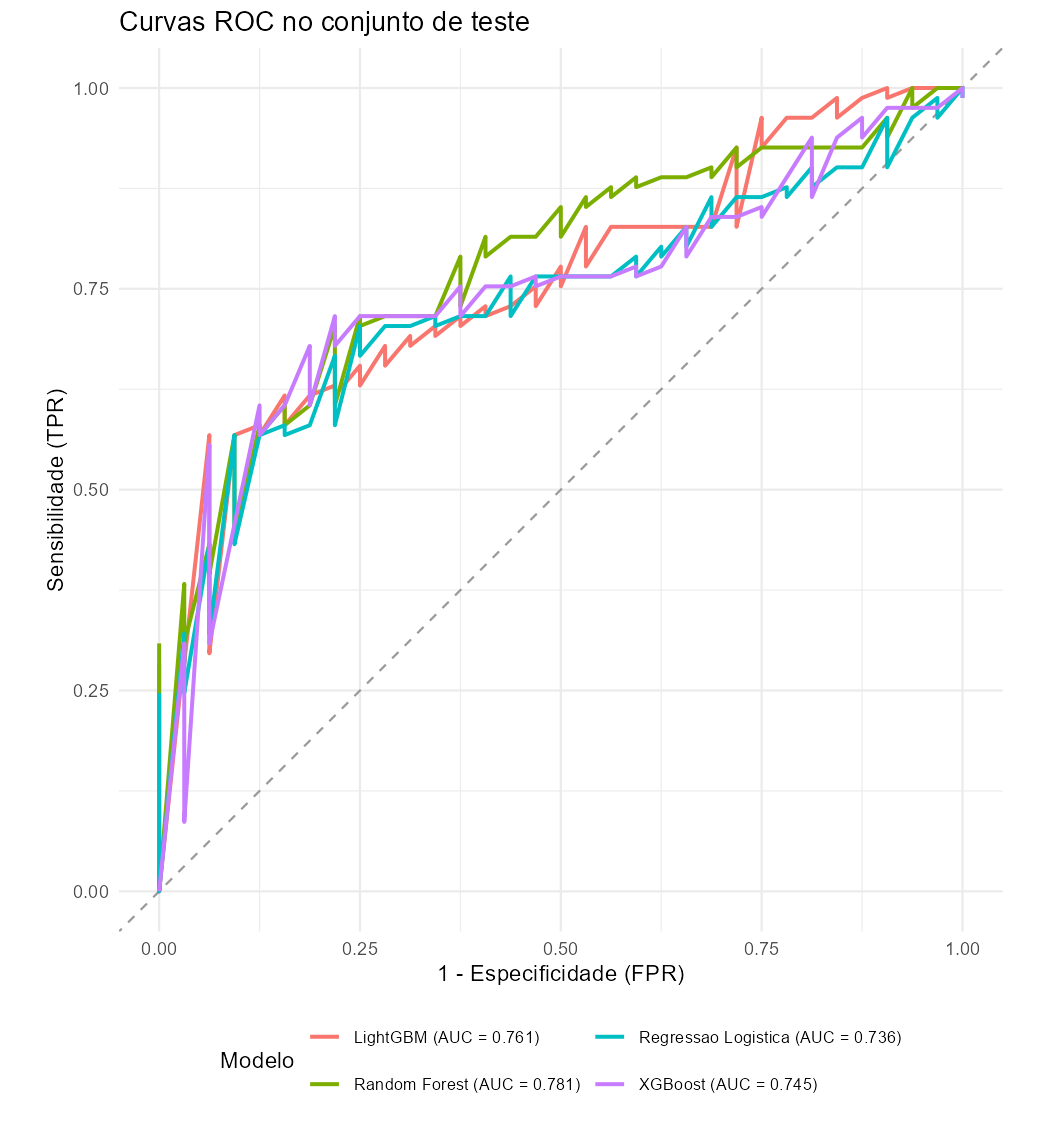
\includegraphics[width=0.6\textwidth]{figuras/cap5-resultados/roc_teste.png}
\caption{Curvas ROC dos quatro modelos no conjunto de teste. A diagonal tracejada representa um classificador aleatório.}
\label{fig:res_roc}
\end{figure}

\subsection{Análise do Limiar de Decisão}
\label{sec:res_limiar}

Os limiares clínicos ficaram entre 0,320 e 0,375 (Tabela~\ref{tab:res_limiares}). A meta de 90\% de sensibilidade se manteve no teste para a Regressão Logística, o \textit{Random Forest} e o LightGBM (73 de 81 doentes), mas não para o XGBoost (0,840). O custo é alto: a especificidade cai para 0,19 a 0,31 (só 6 a 10 dos 32 saudáveis reconhecidos), e a precisão fica apenas 2 a 5 pontos acima da prevalência de 0,717. No regime de triagem, portanto, os modelos acrescentam pouco em relação a encaminhar todos os pacientes para investigação, algo que a AUC sozinha não revela \cite{VanCalster2025Evaluation}.

\begin{table}[htbp]
\centering
\caption{Desempenho no conjunto de teste com o limiar clínico (sensibilidade $\geq$ 90\% na validação cruzada).}
\label{tab:res_limiares}
\begin{tabular}{lcccc}
\hline
\textbf{Modelo} & \textbf{Limiar} & \textbf{Sens.} & \textbf{Espec.} & \textbf{Prec.} \\
\hline
Reg. Logística         & 0,320 & 0,901 & 0,188 & 0,737 \\
\textit{Random Forest} & 0,375 & 0,901 & 0,313 & 0,768 \\
XGBoost                & 0,361 & 0,840 & 0,313 & 0,756 \\
LightGBM               & 0,360 & 0,901 & 0,281 & 0,760 \\
\hline
\end{tabular}
\end{table}

As probabilidades também não devem ser lidas como riscos reais: o SMOTE aumentou a proporção de saudáveis no treino, e a probabilidade média prevista pelo \textit{Random Forest} no teste (0,654) ficou abaixo da proporção real de doentes (0,717). A reamostragem tende a descalibrar os modelos sem melhorar a discriminação \cite{vandenGoorbergh2022Harm, Carriero2025Harms}; a calibração não foi avaliada neste trabalho.

% =============================================================================
\section{Avaliação Estratificada por Sexo}
\label{sec:res_sexo}
% =============================================================================

No teste, 17 das 32 mulheres (53,1\%) e 64 dos 81 homens (79,0\%) eram doentes. As diferenças de AUC entre os sexos foram pequenas, de $-0{,}043$ a $+0{,}019$ (Tabela~\ref{tab:res_sexo}), e os intervalos das mulheres têm o dobro da amplitude dos do conjunto completo. A taxa de falsos negativos foi maior entre as mulheres apenas no XGBoost (0,353 contra 0,266, diferença de cerca de dois pacientes) e menor nos outros três modelos. No limiar clínico, a meta de 90\% nem sempre foi atingida nos dois grupos: na Regressão Logística e no LightGBM, todas as mulheres doentes foram identificadas, mas os homens ficaram em 0,875.

\begin{table}[htbp]
\centering
\caption{Desempenho no conjunto de teste por sexo (F: 32 pacientes, 17 doentes; M: 81 pacientes, 64 doentes).}
\label{tab:res_sexo}
\small
\begin{tabular}{llcccccc}
\hline
 & & & \multicolumn{3}{c}{\textbf{Limiar padrão}} & \multicolumn{2}{c}{\textbf{Limiar clínico}} \\
\textbf{Modelo} & \textbf{Sexo} & \textbf{AUC-ROC [IC 95\%]} & \textbf{Sens.} & \textbf{Espec.} & \textbf{Taxa FN} & \textbf{Sens.} & \textbf{Espec.} \\
\hline
Reg. Logística         & F & 0,729 [0,546; 0,913] & 0,765 & 0,467 & 0,235 & 1,000 & 0,133 \\
                       & M & 0,748 [0,628; 0,868] & 0,719 & 0,647 & 0,281 & 0,875 & 0,235 \\
\textit{Random Forest} & F & 0,790 [0,619; 0,961] & 0,824 & 0,667 & 0,176 & 0,882 & 0,200 \\
                       & M & 0,781 [0,669; 0,894] & 0,766 & 0,588 & 0,234 & 0,906 & 0,412 \\
XGBoost                & F & 0,733 [0,551; 0,916] & 0,647 & 0,733 & 0,353 & 0,824 & 0,333 \\
                       & M & 0,743 [0,615; 0,870] & 0,734 & 0,706 & 0,266 & 0,844 & 0,294 \\
LightGBM               & F & 0,780 [0,618; 0,943] & 0,706 & 0,800 & 0,294 & 1,000 & 0,267 \\
                       & M & 0,737 [0,616; 0,858] & 0,688 & 0,529 & 0,313 & 0,875 & 0,294 \\
\hline
\multicolumn{8}{l}{\footnotesize Taxa FN: proporção de doentes classificados como saudáveis (1 $-$ sensibilidade).} \\
\end{tabular}
\end{table}

Esses resultados não reproduzem a disparidade relatada por \citeonline{investigatingbiashealth}, que encontraram taxas de falsos negativos cerca de 20 pontos maiores nas mulheres. A explicação mais simples é o tamanho da amostra: com 17 mulheres doentes, este trabalho não consegue confirmar nem descartar diferenças dessa magnitude, e a ausência de disparidade não deve ser lida como evidência de equidade \cite{Rajkomar2018Ensuring}.

% =============================================================================
\section{Interpretabilidade com SHAP}
\label{sec:res_shap}
% =============================================================================

O valor base, previsão média no teste a partir da qual as contribuições são somadas, foi de 0,167 log-odds no XGBoost (probabilidade de cerca de 0,54), 0,304 no LightGBM (cerca de 0,58) e 0,654 em probabilidade no \textit{Random Forest}.

\subsection{Importância Global}
\label{sec:res_shap_global}

Os três modelos concordam que as bilirrubinas, a fosfatase alcalina e as aminotransferases são as variáveis mais relevantes e que o sexo é pouco relevante, mas distribuem a importância de formas muito diferentes (Tabela~\ref{tab:res_shap_imp}).

\begin{table}[htbp]
\centering
\caption{Importância SHAP global (média dos valores SHAP absolutos no teste): posição no ranking e participação percentual na importância total.}
\label{tab:res_shap_imp}
\begin{tabular}{lcccccc}
\hline
 & \multicolumn{2}{c}{\textbf{XGBoost}} & \multicolumn{2}{c}{\textbf{LightGBM}} & \multicolumn{2}{c}{\textbf{\textit{Random Forest}}} \\
\textbf{Variável} & \textbf{Pos.} & \textbf{\%} & \textbf{Pos.} & \textbf{\%} & \textbf{Pos.} & \textbf{\%} \\
\hline
Total\_Bilirubin            & 1     & 37,6 & 4  & 16,5 & 3  & 13,8 \\
Alkaline\_Phosphotase       & 2     & 26,4 & 1  & 23,0 & 1  & 18,4 \\
Total\_Proteins             & 3     & 8,5  & 9  & 0,7  & 9  & 4,9 \\
Aspartate\_Aminotransferase & 4     & 8,1  & 3  & 16,8 & 5  & 11,8 \\
Age                         & 5     & 7,9  & 6  & 7,3  & 6  & 8,1 \\
AG\_Ratio                   & 6     & 5,8  & 7  & 5,4  & 7  & 7,3 \\
Alamine\_Aminotransferase   & 7     & 5,6  & 5  & 9,1  & 4  & 12,0 \\
Direct\_Bilirubin           & 8--10 & 0,0  & 2  & 19,2 & 2  & 14,7 \\
Albumin                     & 8--10 & 0,0  & 8  & 2,1  & 8  & 6,0 \\
Gender                      & 8--10 & 0,0  & 10 & 0,0  & 10 & 3,1 \\
\hline
\multicolumn{7}{l}{\footnotesize Variáveis não utilizadas por um modelo têm importância nula e empatam nas últimas posições.} \\
\end{tabular}
\end{table}

No XGBoost, a importância é concentrada: bilirrubina total e fosfatase alcalina somam 64\%, e \textit{Direct\_Bilirubin}, \textit{Albumin} e \textit{Gender} têm importância nula porque não aparecem em nenhuma árvore. Com poucas árvores e forte regularização (Tabela~\ref{tab:res_hiper}), o modelo faz poucas divisões e, entre variáveis redundantes, usa apenas uma: a bilirrubina total em vez da direta, e \textit{Total\_Proteins} e \textit{AG\_Ratio}, que juntas determinam a albumina. No \textit{Random Forest}, ao contrário, a importância é distribuída: as cinco primeiras variáveis têm entre 11,8\% e 18,4\%. Com \texttt{mtry} = 1, o modelo alterna entre variáveis correlacionadas e divide o crédito entre elas, comportamento conhecido tanto para o \textit{Random Forest} \cite{Strobl2008Conditional} quanto para o SHAP \cite{Aas2021Explaining}. O LightGBM, embora seja de \textit{boosting} como o XGBoost, se parece mais com o \textit{Random Forest}: suas muitas árvores pequenas acabam usando as duas variáveis de cada par, mas ele praticamente ignora as proteínas e não usa \textit{Gender}.

As cinco variáveis mais importantes no \textit{Random Forest} e no LightGBM são exatamente as cinco cuja média mais difere entre as classes (Tabela~\ref{tab:medias_classe}). Já no XGBoost, \textit{Total\_Proteins}, que quase não difere entre as classes, ficou em terceiro, o que indica um papel condicional às demais variáveis. Cada retrato descreve corretamente o seu modelo, mas, juntos, mostram que a importância de uma variável depende também do algoritmo e dos hiperparâmetros.

\subsection{Direção e Forma dos Efeitos}
\label{sec:res_shap_direcao}

Os \textit{beeswarms} (Figura~\ref{fig:res_beeswarm}) e as correlações entre o valor e o SHAP de cada variável (Tabela~\ref{tab:res_direcao}) mostram efeitos no mesmo sentido nos três modelos: valores altos de bilirrubinas, fosfatase alcalina, aminotransferases e idade aumentam a previsão de doença, e valores altos de \textit{AG\_Ratio} (e de albumina, no \textit{Random Forest}) a reduzem. Esses sentidos são coerentes com a clínica \cite{Kwo2016ACG, Trebicka2025Controversies}, o que não prova causalidade, mas indica que os modelos não se apoiam em padrões espúrios.

\begin{figure}[htbp]
\centering
\begin{minipage}{0.49\textwidth}
\centering
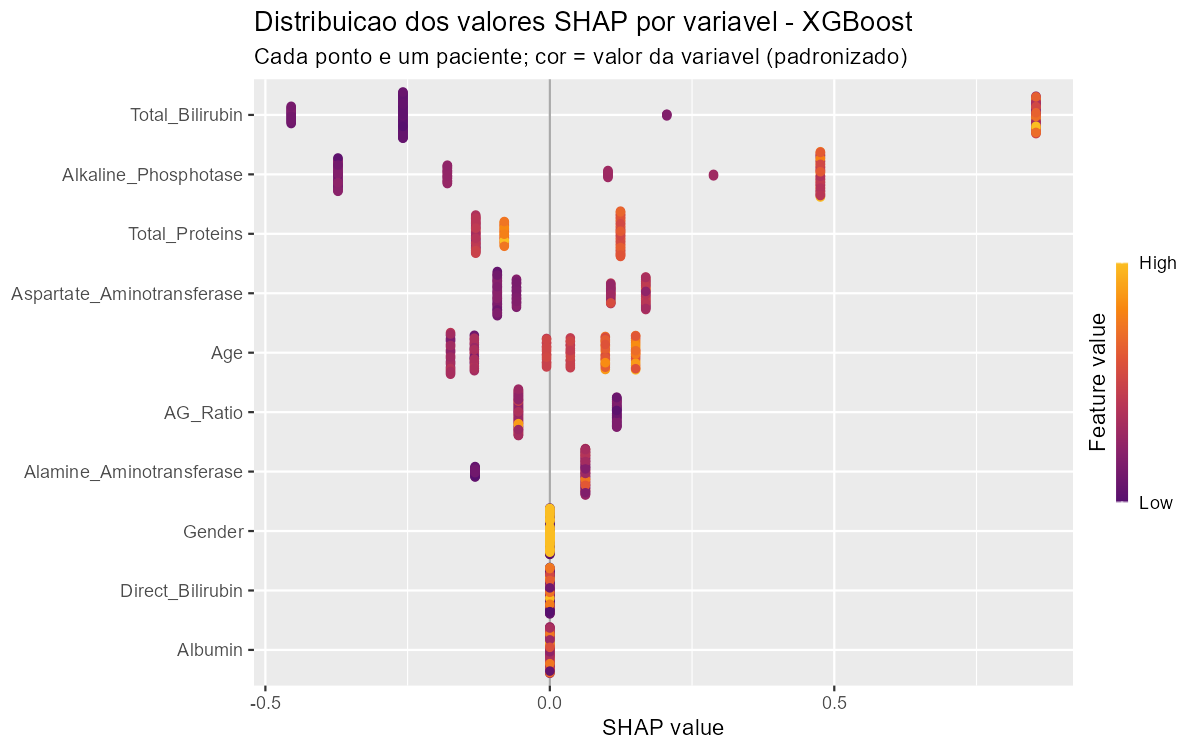
\includegraphics[width=\textwidth]{figuras/cap5-resultados/shap_beeswarm_xgb.png}\\
\small (a) XGBoost
\end{minipage}
\hfill
\begin{minipage}{0.49\textwidth}
\centering
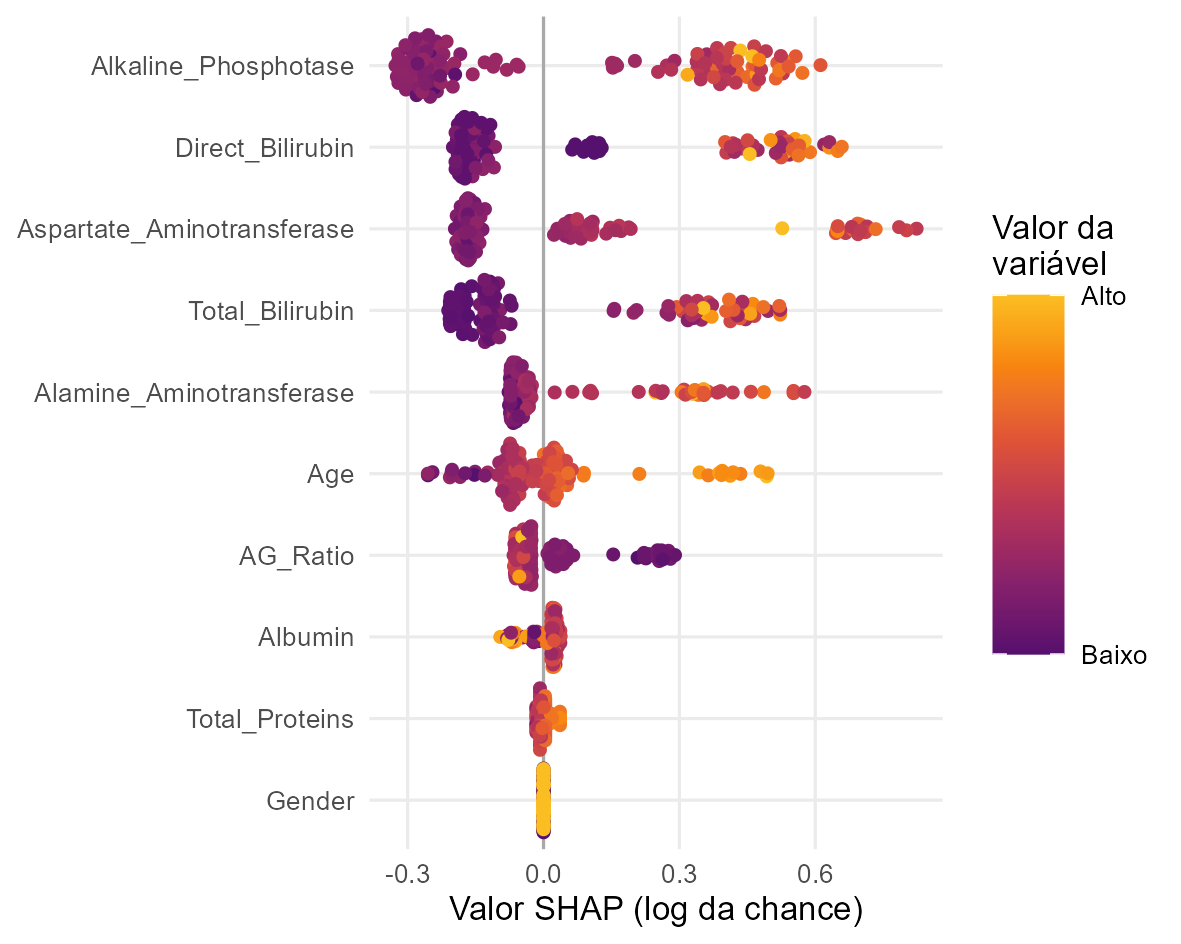
\includegraphics[width=\textwidth]{figuras/cap5-resultados/shap_beeswarm_lgb.png}\\
\small (b) LightGBM
\end{minipage}

\vspace{0.3cm}

\begin{minipage}{0.49\textwidth}
\centering
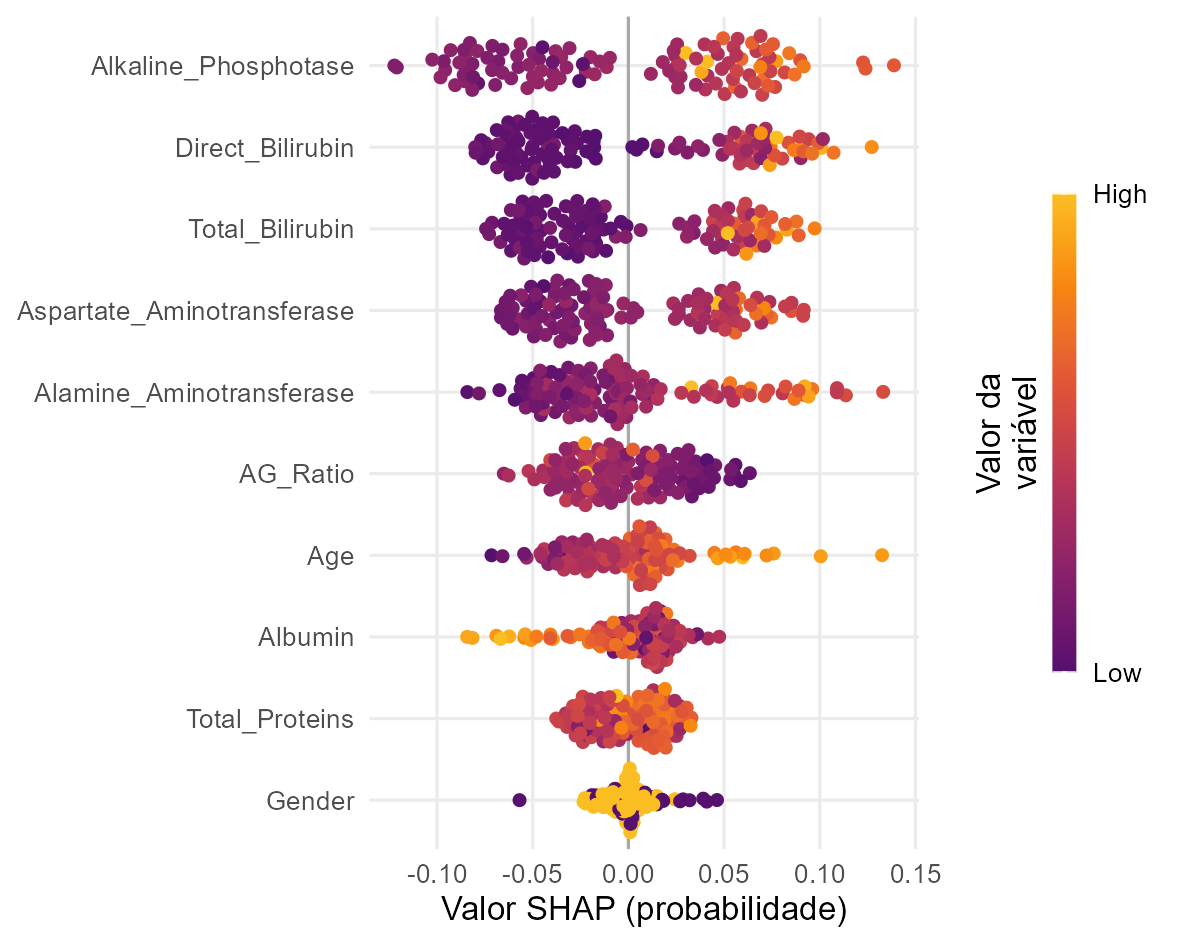
\includegraphics[width=\textwidth]{figuras/cap5-resultados/shap_beeswarm_rf.png}\\
\small (c) \textit{Random Forest}
\end{minipage}
\caption{Valores SHAP por variável no conjunto de teste. Cada ponto é um paciente, colorido do menor ao maior valor da variável; pontos à direita do zero aumentam a previsão de doença.}
\label{fig:res_beeswarm}
\end{figure}

\begin{table}[htbp]
\centering
\caption{Correlação de Pearson entre o valor de cada variável e seu valor SHAP no conjunto de teste.}
\label{tab:res_direcao}
\begin{tabular}{lccc}
\hline
\textbf{Variável} & \textbf{XGBoost} & \textbf{LightGBM} & \textbf{\textit{Random Forest}} \\
\hline
Age                         & 0,860      & 0,868      & 0,894 \\
Total\_Bilirubin            & 0,807      & 0,864      & 0,855 \\
Direct\_Bilirubin           & ---        & 0,819      & 0,818 \\
Alkaline\_Phosphotase       & 0,810      & 0,816      & 0,754 \\
Alamine\_Aminotransferase   & 0,531      & 0,791      & 0,841 \\
Aspartate\_Aminotransferase & 0,717      & 0,874      & 0,824 \\
Total\_Proteins             & 0,360      & 0,770      & 0,425 \\
Albumin                     & ---        & $-0{,}046$ & $-0{,}737$ \\
AG\_Ratio                   & $-0{,}669$ & $-0{,}668$ & $-0{,}572$ \\
Gender                      & ---        & ---        & $-0{,}140$ \\
\hline
\multicolumn{4}{l}{\footnotesize ---: variável não utilizada pelo modelo (valores SHAP constantes).} \\
\end{tabular}
\end{table}

A forma dos efeitos difere (Figura~\ref{fig:res_dependencia}). No XGBoost, cada variável participa de poucas divisões, e o efeito é em degraus: na bilirrubina total, pacientes a partir de cerca de 1,8~mg/dL recebem $+0{,}86$ log-odds, e um paciente com 1,6~mg/dL já recebe $-0{,}45$. Em \textit{Total\_Proteins}, o efeito não é monotônico (valores intermediários aumentam a previsão), o que explica sua correlação fraca e provavelmente funciona como substituto da albumina, mas é difícil de traduzir em regra clínica. No LightGBM e no \textit{Random Forest}, cuja variável mais importante é a fosfatase alcalina, a curva tem forma de ``S'', quase um degrau no LightGBM e mais gradual no \textit{Random Forest}.

\begin{figure}[htbp]
\centering
\begin{minipage}{0.49\textwidth}
\centering
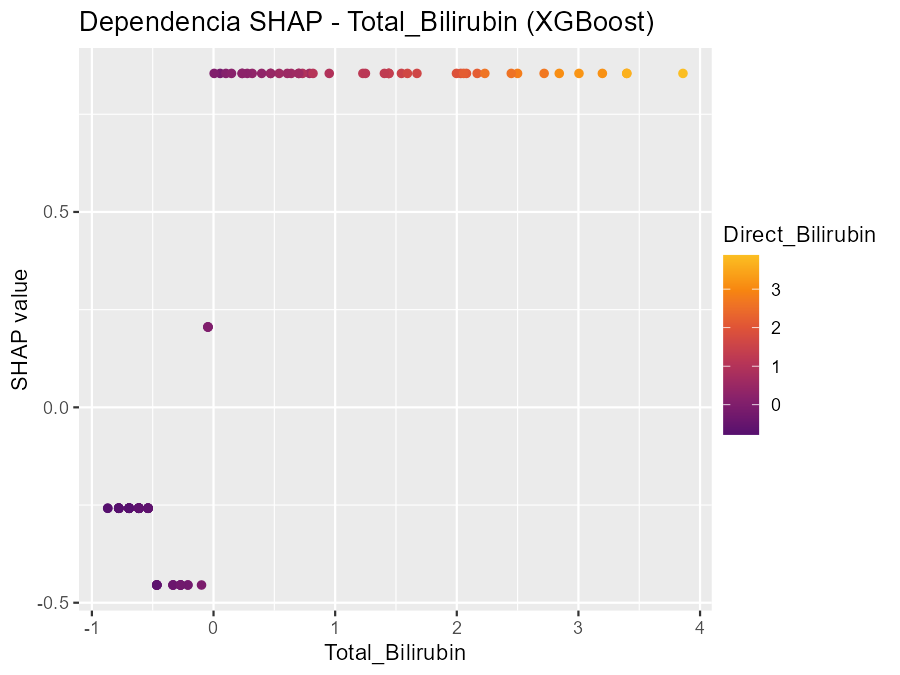
\includegraphics[width=\textwidth]{figuras/cap5-resultados/shap_dependencia_xgb_Total_Bilirubin.png}\\
\small (a) XGBoost: \textit{Total\_Bilirubin}
\end{minipage}
\hfill
\begin{minipage}{0.49\textwidth}
\centering
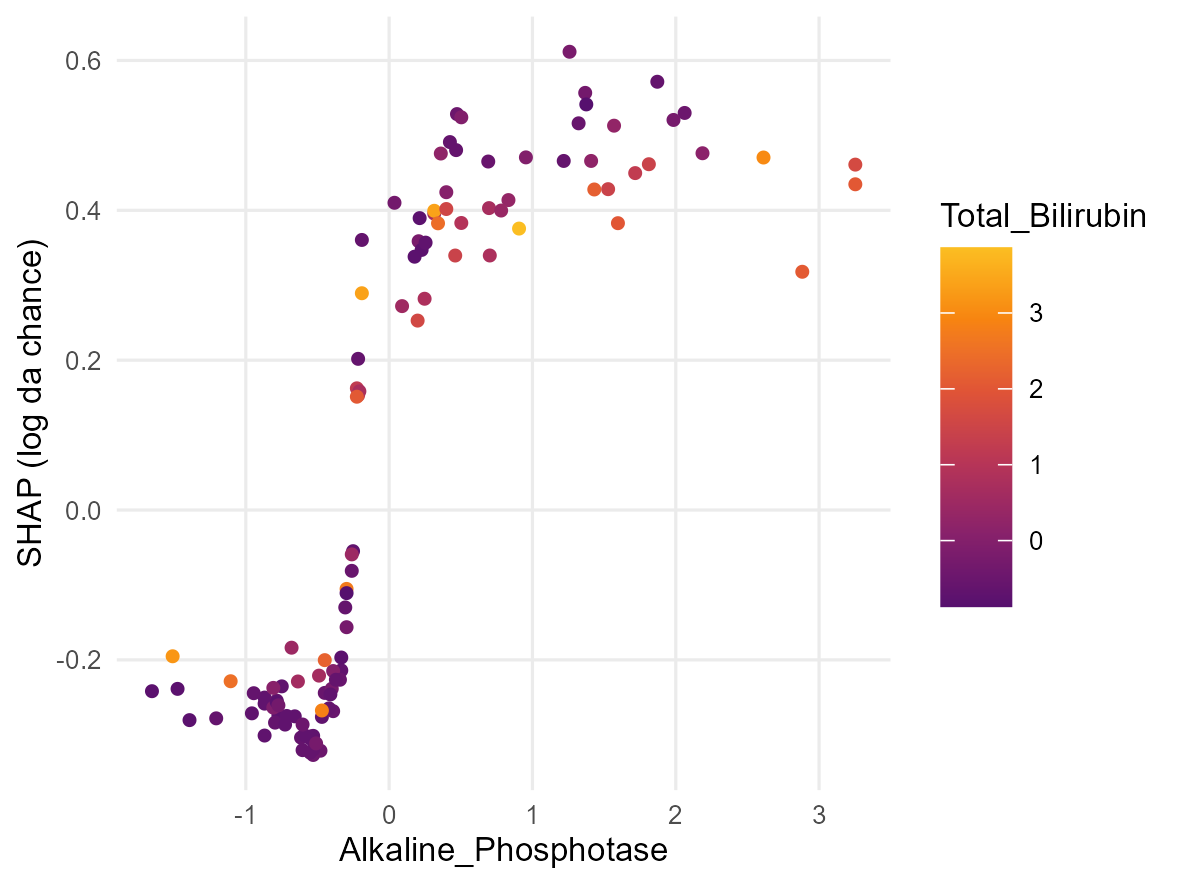
\includegraphics[width=\textwidth]{figuras/cap5-resultados/shap_dependencia_lgb_Alkaline_Phosphotase.png}\\
\small (b) LightGBM: \textit{Alkaline\_Phosphotase}
\end{minipage}

\vspace{0.3cm}

\begin{minipage}{0.49\textwidth}
\centering
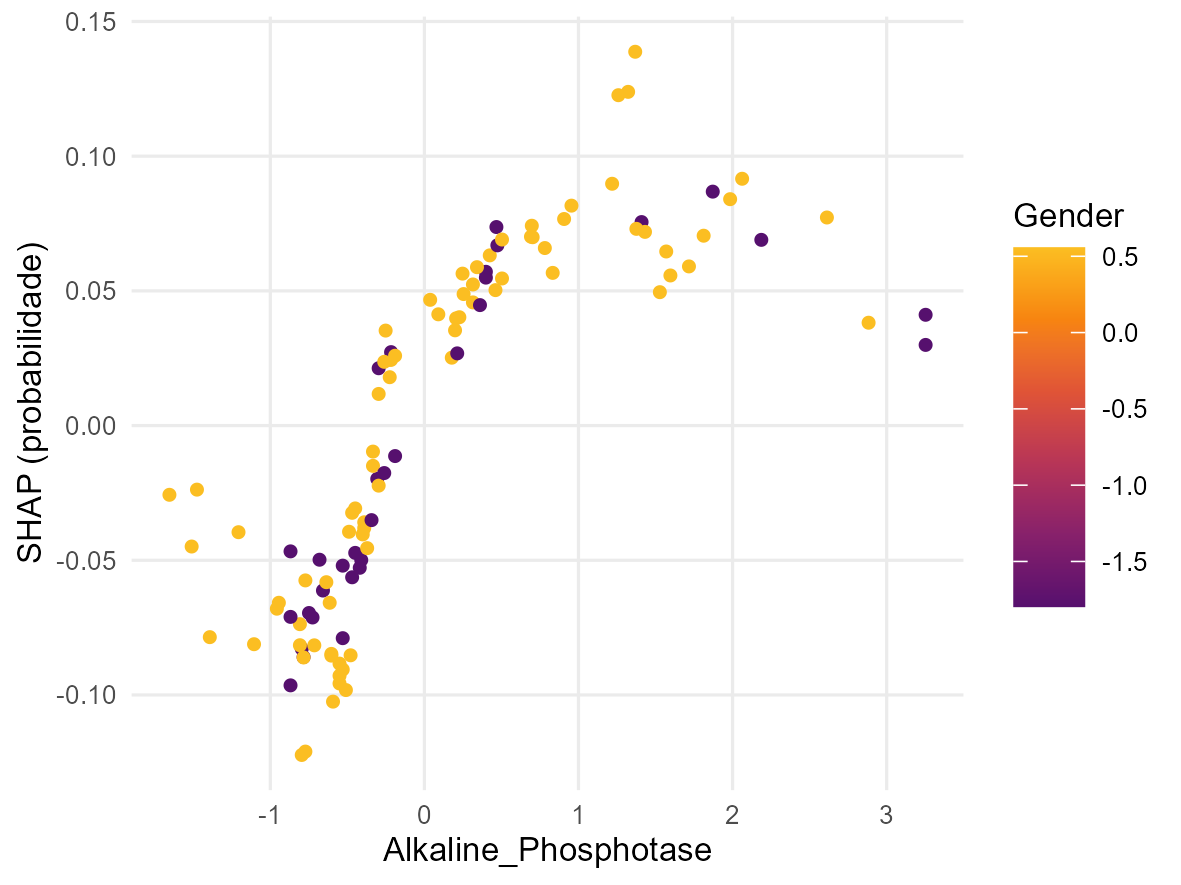
\includegraphics[width=\textwidth]{figuras/cap5-resultados/shap_dependencia_rf_Alkaline_Phosphotase.png}\\
\small (c) \textit{Random Forest}: \textit{Alkaline\_Phosphotase}
\end{minipage}
\caption{Gráficos de dependência SHAP da variável mais importante de cada modelo (eixo horizontal na escala padronizada).}
\label{fig:res_dependencia}
\end{figure}

\subsection{Explicações Locais}
\label{sec:res_shap_local}

Nos verdadeiros positivos de maior confiança, os três modelos se apoiaram nos mesmos exames, muito acima das medianas da base: por exemplo, no LightGBM, um homem de 66 anos com AST de 4.929~IU/L (o maior valor da base) recebeu probabilidade de 0,92. Os valores dos exames citados nesta seção foram convertidos para as unidades originais.

Os falsos negativos de pior erro (Figura~\ref{fig:res_waterfall_fn}) são mais reveladores. No XGBoost, um homem de 35 anos recebeu probabilidade de apenas 0,224: sua bilirrubina total (1,6~mg/dL) ficou logo abaixo do degrau de 1,8~mg/dL e gerou a maior contribuição para ``saudável'', enquanto sua albumina baixa (2,5~g/dL), um possível sinal de doença, não teve efeito porque o modelo não usa essa variável. No LightGBM, um homem de 30 anos (probabilidade de 0,334) também tinha albumina (2,3~g/dL) e proteínas totais (4,6~g/dL) baixas, sinais que o modelo praticamente ignora. Esses casos mostram que um modelo que descarta variáveis \emph{em média} pode descartar justamente a informação decisiva para um paciente.

\begin{figure}[htbp]
\centering
\begin{minipage}{0.49\textwidth}
\centering
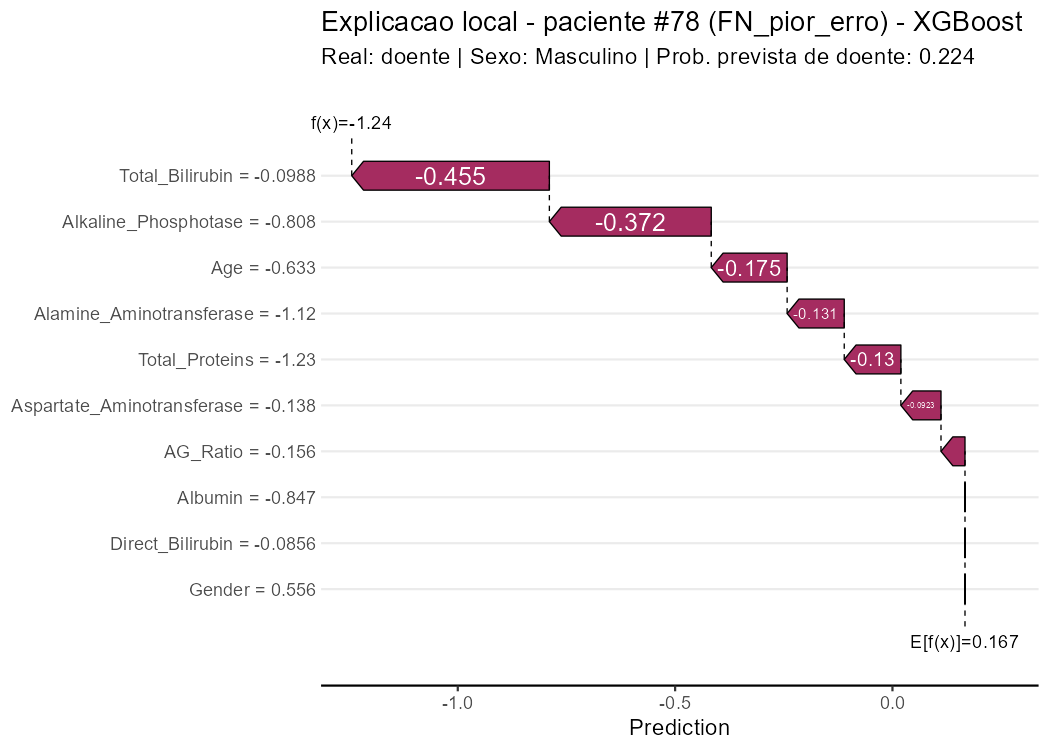
\includegraphics[width=\textwidth]{figuras/cap5-resultados/shap_waterfall_xgb_FN_pior_erro.png}\\
\small (a) XGBoost
\end{minipage}
\hfill
\begin{minipage}{0.49\textwidth}
\centering
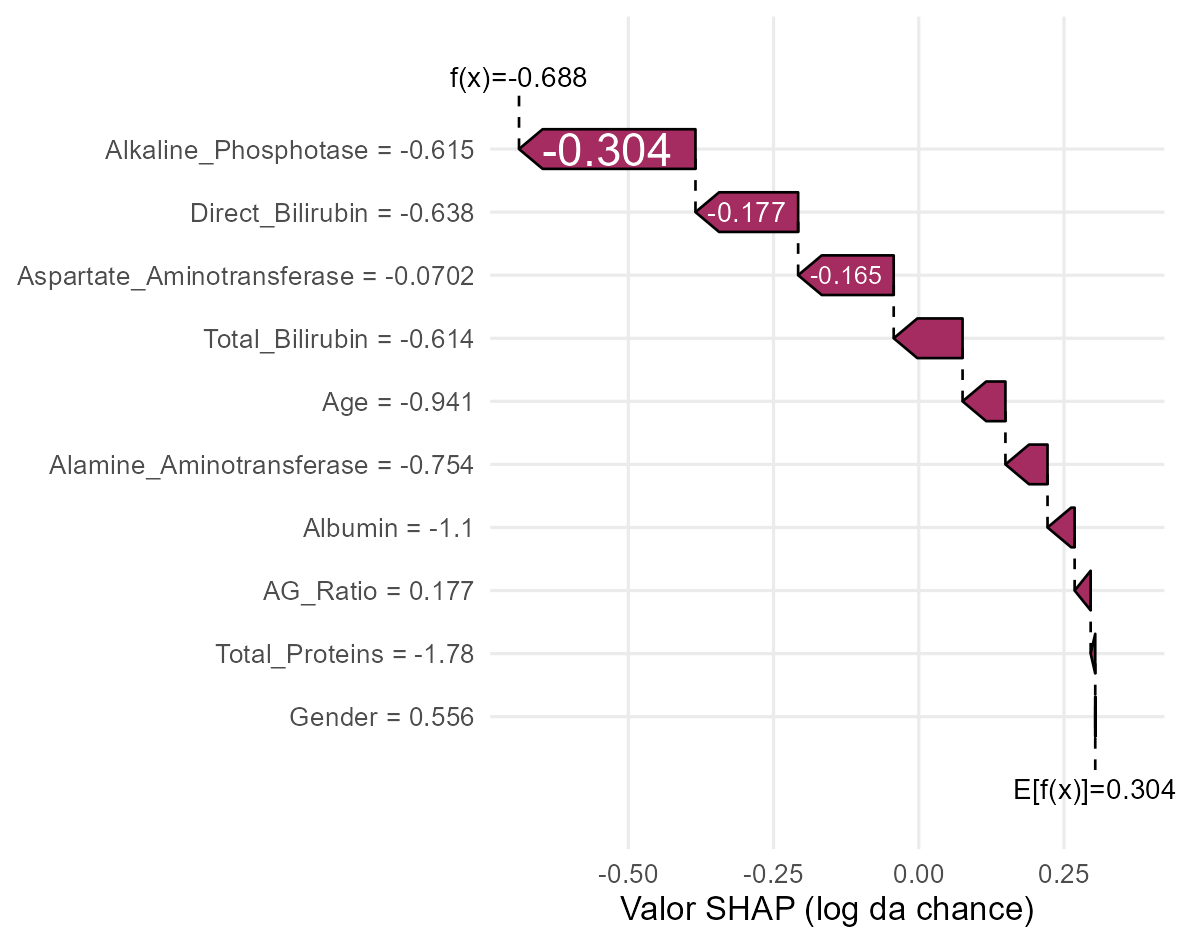
\includegraphics[width=\textwidth]{figuras/cap5-resultados/shap_waterfall_lgb_FN_pior_erro.png}\\
\small (b) LightGBM
\end{minipage}

\vspace{0.3cm}

\begin{minipage}{0.49\textwidth}
\centering
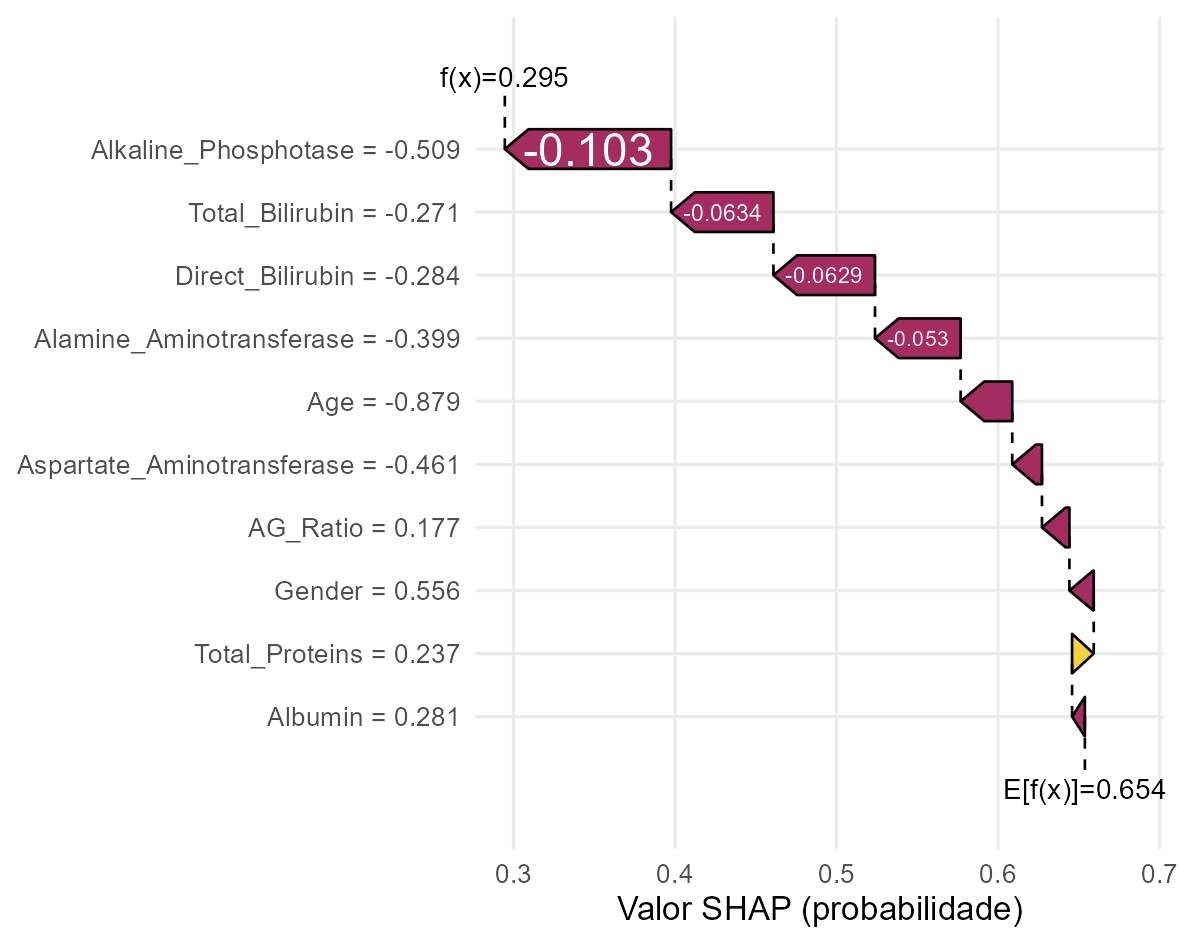
\includegraphics[width=\textwidth]{figuras/cap5-resultados/shap_waterfall_rf_FN_pior_erro.png}\\
\small (c) \textit{Random Forest}
\end{minipage}
\caption{Explicações locais dos falsos negativos de pior erro (pacientes doentes classificados com maior confiança como saudáveis).}
\label{fig:res_waterfall_fn}
\end{figure}

No \textit{Random Forest}, o falso negativo de pior erro (homem de 31 anos, probabilidade de 0,248) tinha exames compatíveis com os de um paciente saudável, como ALT de 29~IU/L, abaixo do limite de 42~IU/L proposto para homens por \citeonline{Valenti2021Definition}. Aqui, o erro parece vir da própria informação disponível, já que a doença hepática pode existir com exames normais \cite{Lominadze2018Misconception}. As explicações locais permitem, assim, distinguir erros causados pelas escolhas do modelo de erros que nenhum modelo baseado nesses atributos evitaria. Como os valores SHAP do \textit{Random Forest} são estimados por amostragem, sua soma não reproduz exatamente a previsão (0,295 contra 0,248 nesse paciente), e contribuições pequenas devem ser lidas com cautela.

\subsection{Auditoria de Viés por Sexo}
\label{sec:res_shap_sexo}

A importância das variáveis foi muito semelhante entre os sexos (Figura~\ref{fig:res_shap_sexo}): a correlação de Spearman entre os rankings de homens e mulheres foi de 0,988 nos três modelos, com apenas trocas entre variáveis vizinhas. O XGBoost e o LightGBM não usam \textit{Gender}. No \textit{Random Forest}, \textit{Gender} é a variável menos importante, e sua contribuição média foi de $+0{,}0030$ nas mulheres e $-0{,}0015$ nos homens (Figura~\ref{fig:res_shap_gender}), no mesmo sentido do coeficiente da Regressão Logística, mas menor que meio ponto percentual. A auditoria não encontrou, portanto, indício de que os modelos usem o sexo como atalho ou se apoiem em variáveis diferentes para cada grupo, com as mesmas limitações de tamanho amostral já discutidas.

\begin{figure}[htbp]
\centering
\begin{minipage}{0.49\textwidth}
\centering
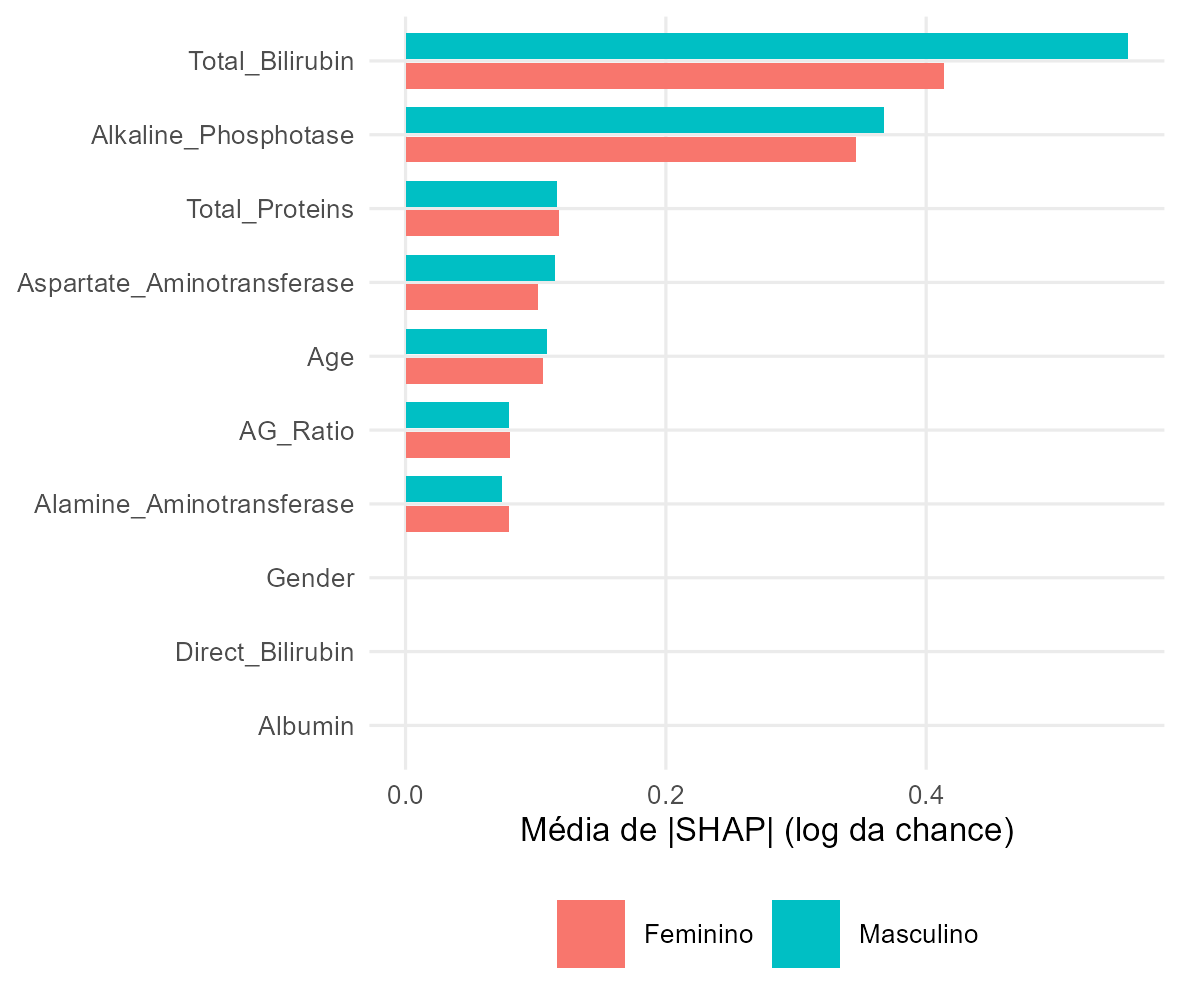
\includegraphics[width=\textwidth]{figuras/cap5-resultados/shap_importancia_por_sexo_xgb.png}\\
\small (a) XGBoost
\end{minipage}
\hfill
\begin{minipage}{0.49\textwidth}
\centering
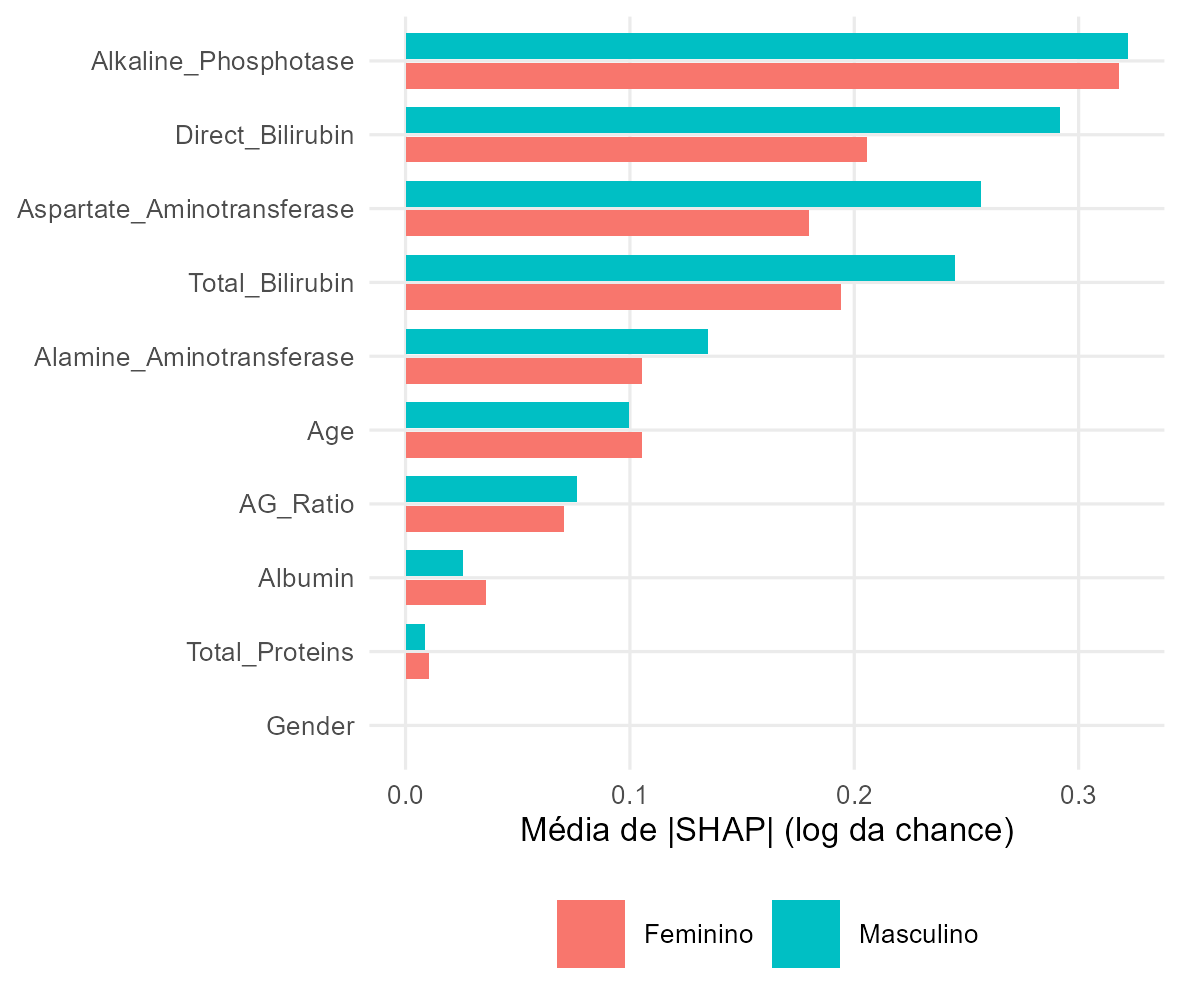
\includegraphics[width=\textwidth]{figuras/cap5-resultados/shap_importancia_por_sexo_lgb.png}\\
\small (b) LightGBM
\end{minipage}

\vspace{0.3cm}

\begin{minipage}{0.49\textwidth}
\centering
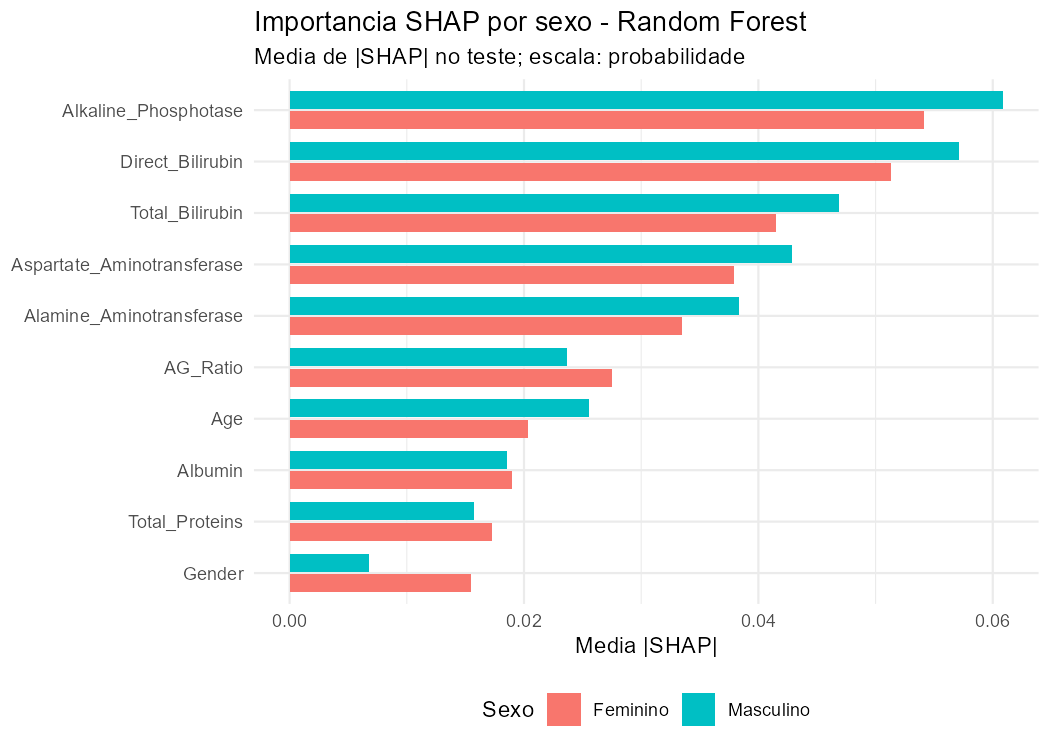
\includegraphics[width=\textwidth]{figuras/cap5-resultados/shap_importancia_por_sexo_rf.png}\\
\small (c) \textit{Random Forest}
\end{minipage}
\caption{Importância SHAP global calculada separadamente para os pacientes de cada sexo no conjunto de teste.}
\label{fig:res_shap_sexo}
\end{figure}

\begin{figure}[htbp]
\centering
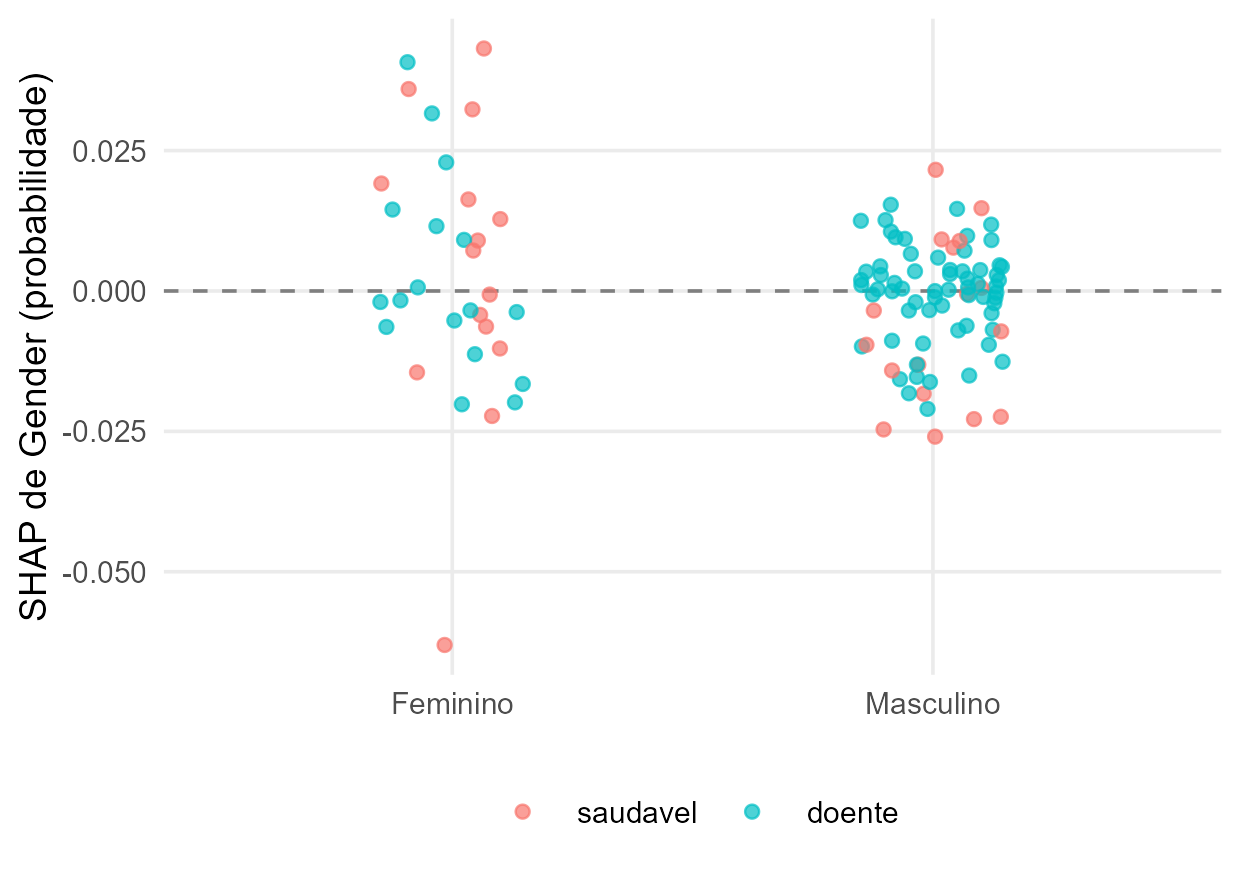
\includegraphics[width=0.55\textwidth]{figuras/cap5-resultados/shap_gender_por_sexo_rf.png}
\caption{Contribuição SHAP da variável \textit{Gender} no \textit{Random Forest}, por sexo e classe real. Valores positivos aumentam a probabilidade prevista de doença.}
\label{fig:res_shap_gender}
\end{figure}

\subsection{Comparação das Importâncias entre os Modelos}
\label{sec:res_comparacao_importancias}

Os rankings do LightGBM e do \textit{Random Forest} foram quase idênticos ($\rho = 0{,}96$), embora um use \textit{boosting} e o outro \textit{bagging}; o do XGBoost concordou pouco com ambos ($\rho = 0{,}36$), e o da Regressão Logística teve correlação negativa com todos (Tabela~\ref{tab:res_rankings}). O ranking da Regressão Logística é dominado pelas proteínas, cujos coeficientes são grandes porque se compensam (Seção~\ref{sec:res_coef_lr}), e não por serem as mais informativas \cite{Dormann2013Collinearity}. O XGBoost se afasta dos outros dois porque escolheu uma variável de cada par redundante, enquanto os demais dividiram o crédito. A distribuição da importância depende, portanto, mais da configuração do modelo do que da estratégia de \textit{ensemble}.

\begin{table}[htbp]
\centering
\caption{Posição de cada variável nos quatro rankings de importância (1 = mais importante).}
\label{tab:res_rankings}
\begin{tabular}{lcccc}
\hline
 & \multicolumn{3}{c}{\textbf{SHAP}} & \textbf{$|$Coef.$|$} \\
\textbf{Variável} & \textbf{XGB} & \textbf{LGB} & \textbf{RF} & \textbf{RL} \\
\hline
Total\_Bilirubin            & 1 & 4  & 3  & 9 \\
Alkaline\_Phosphotase       & 2 & 1  & 1  & 5 \\
Total\_Proteins             & 3 & 9  & 9  & 2 \\
Aspartate\_Aminotransferase & 4 & 3  & 5  & 8 \\
Age                         & 5 & 6  & 6  & 7 \\
AG\_Ratio                   & 6 & 7  & 7  & 3 \\
Alamine\_Aminotransferase   & 7 & 5  & 4  & 4 \\
Direct\_Bilirubin           & 9 & 2  & 2  & 6 \\
Albumin                     & 9 & 8  & 8  & 1 \\
Gender                      & 9 & 10 & 10 & 10 \\
\hline
\multicolumn{5}{l}{\footnotesize XGB: XGBoost; LGB: LightGBM; RF: \textit{Random Forest}; RL: Regressão Logística.} \\
\multicolumn{5}{l}{\footnotesize Empates recebem o posto médio. Spearman: XGB--LGB $= 0{,}362$; XGB--RF $= 0{,}362$;} \\
\multicolumn{5}{l}{\footnotesize LGB--RF $= 0{,}964$; XGB--RL $= -0{,}141$; LGB--RL $= -0{,}200$; RF--RL $= -0{,}164$.} \\
\end{tabular}
\end{table}

Alguns resultados se repetem em todos os modelos: uma das bilirrubinas e a fosfatase alcalina estão sempre entre as mais importantes nos três \textit{ensembles}, e \textit{Gender} fica nas últimas posições nos quatro rankings. São esses resultados estáveis, e não a posição exata de cada variável, que podem ser afirmados com segurança. Modelos com desempenho estatisticamente indistinguível podem oferecer explicações bem diferentes dos mesmos dados, o chamado efeito Rashomon \cite{Biecek2024Performance}, e a interpretação de um único modelo não deve ser tomada como descrição definitiva da relação entre os exames e a doença.

% =============================================================================
\section{Síntese dos Resultados}
\label{sec:res_sintese}
% =============================================================================

\begin{enumerate}
    \item \textit{Desempenho}: nenhum \textit{ensemble} superou a Regressão Logística de forma significativa; as AUCs (0,74 a 0,79) indicam discriminação moderada, com intervalos largos.
    \item \textit{Limiar}: exigir 90\% de sensibilidade reduz a especificidade a 0,19--0,31, e os modelos acrescentam pouco à triagem de todos os pacientes.
    \item \textit{Sexo}: não houve disparidade consistente de desempenho nem de uso das variáveis, mas o subgrupo feminino é pequeno demais para descartá-la.
    \item \textit{Interpretabilidade}: os efeitos estimados pelo SHAP são coerentes com a clínica, mas a importância das variáveis depende do modelo e dos hiperparâmetros, sobretudo entre variáveis correlacionadas.
    \item \textit{Explicações locais}: os falsos negativos permitiram distinguir erros causados pelo modelo (descarte das proteínas no XGBoost e no LightGBM) de erros inevitáveis com esses atributos.
\end{enumerate}

Como limitações, o teste é pequeno e vem de uma única divisão \cite{Vergouwe2005Substantial}, a calibração e a utilidade clínica não foram avaliadas \cite{Vickers2006Decision}, e os valores SHAP do \textit{Random Forest} são aproximações. Esses pontos são retomados na Conclusão.
